% Section 3: Experimental Setup
% Note: \section{} header is in main.tex

\subsection{Iterative Self-Training Pipeline}
\label{sec:pipeline}

\begin{figure}[t]
\centering
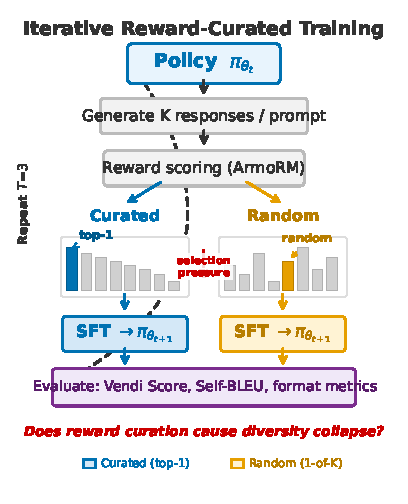
\includegraphics[width=\columnwidth]{figures/fig1_pipeline.pdf}
\caption{Iterative self-training pipeline. Each generation generates $K$ candidates per prompt, scores them with ArmoRM, selects the top-1, and fine-tunes the base model for the next generation.}
\label{fig:pipeline}
\end{figure}

We study diversity dynamics through an iterative self-training loop (Figure~\ref{fig:pipeline}). The base model is Qwen3-0.6B \cite{placeholder_qwen3} (596M parameters), chosen as the smallest model capable of coherent instruction-following in tractable compute budgets. We use UltraFeedback \cite{placeholder_ultrafeedback} as the prompt source, sampling 2{,}200 general instruction-following prompts (2{,}000 train, 200 eval). Each generation proceeds in four steps: (1) generate $K$ candidate responses per prompt; (2) score with ArmoRM-Llama3-8B-v0.1 \cite{placeholder_armorm}; (3) select the top-1 candidate; (4) fine-tune the base model on the selected subset. We run three complete generations (Gen~0 $\rightarrow$ Gen~1 $\rightarrow$ Gen~2). Gen~0 metrics reflect the model after the first training round, not the unmodified base model. All candidate generation uses temperature $T{=}0.7$.

\subsection{Experimental Conditions}
\label{sec:conditions}

Table~\ref{tab:conditions} summarizes the eight configurations. Our design isolates four factors through controlled comparisons. First, adaptation method (LoRA vs.\ Full Fine-Tuning) isolates the effect of parameter capacity: LoRA \cite{placeholder_lora} updates only 1.67\% of parameters (rank 16), while Full-FT (Full Fine-Tuning) updates all parameters. Second, candidate pool size ($K \in \{4, 8, 16\}$) isolates selection pressure, corresponding to 25\%, 12.5\%, and 6.25\% retention rates respectively. Third, learning rate (5e-6 vs.\ 2e-5 for Full-FT) isolates learning intensity across a conservative to aggressive optimization range. Fourth, curation strategy (ArmoRM top-1 vs.\ random selection) isolates the causal effect of reward-based filtering: configurations C5, C6, and C7 serve as matched baselines for C1, C3, and C4 respectively and differ only in whether selection is reward-guided or random.

\begin{table}[t]
\centering
\small
\caption{Experimental configurations. C1--C4 each has a matched random baseline (C5--C7); C8 extends the selection pressure range without a paired baseline. Trainable \% refers to the fraction of model parameters updated during fine-tuning.}
\label{tab:conditions}
\resizebox{\columnwidth}{!}{%
\begin{tabular}{@{}lllcll@{}}
\toprule
ID & Adaptation & $K$ & LR & Curation & Trainable \\
\midrule
C1 & LoRA ($r{=}16$) & 4 & 2e-4 & ArmoRM top-1 & 1.67\% \\
C2 & LoRA ($r{=}16$) & 8 & 2e-4 & ArmoRM top-1 & 1.67\% \\
C3 & Full-FT & 4 & 5e-6 & ArmoRM top-1 & 100\% \\
C4 & Full-FT & 4 & 2e-5 & ArmoRM top-1 & 100\% \\
C8 & Full-FT & 16 & 2e-5 & ArmoRM top-1 & 100\% \\
\midrule
C5 & LoRA ($r{=}16$) & 4 & 2e-4 & Random 1-of-$K$ & 1.67\% \\
C6 & Full-FT & 4 & 5e-6 & Random 1-of-$K$ & 100\% \\
C7 & Full-FT & 4 & 2e-5 & Random 1-of-$K$ & 100\% \\
\bottomrule
\end{tabular}}
\end{table}

This factorial structure enables direct attribution. If reward curation causes diversity collapse, curated conditions (C1--C4, C8) should show steeper diversity decline than their random counterparts (C5--C7) across generations. If parameter capacity mediates collapse, LoRA and Full-FT conditions should diverge even under identical curation. If selection pressure drives collapse, C8 ($K{=}16$, 6.25\% retention) should collapse faster than C2 ($K{=}8$) and C1 ($K{=}4$).

\subsection{Evaluation Metrics}
\label{sec:metrics}

We evaluate diversity at two levels: semantic content and surface format.

\paragraph{Semantic diversity.} Our primary metric is the Vendi Score \cite{placeholder_vendi}, a kernel-based diversity measure computed over sentence embeddings from all-MiniLM-L6-v2 \cite{placeholder_minilm}. The Vendi Score equals the exponential of the Shannon entropy of the eigenvalues of the kernel matrix, with higher values indicating greater diversity. We complement this with Self-BLEU \cite{placeholder_selfbleu}, defined as the average pairwise BLEU score among all responses in the evaluation set (lower indicates more diversity), and Nearest-Neighbor Distance (NND), the average cosine distance to the nearest neighbor in embedding space (higher indicates more diversity). All semantic metrics are computed over the 200 evaluation prompts with one response per prompt per generation.

\paragraph{Format diversity.} Standard embedding-based metrics can miss surface-level homogenization because semantically distinct responses may share identical templates. We introduce two format-level indicators. Opening Entropy measures the Shannon entropy of first-10-token sequences across responses; lower values indicate convergence toward fixed opening patterns. Near-Duplicate Start Rate measures the fraction of response pairs sharing a 50-character prefix; higher values indicate template repetition. These metrics capture a distinct failure mode: models that produce varied content but wrap it in repetitive formatting.

\paragraph{Quality and training dynamics.} We track mean ArmoRM score per generation to verify that quality does not degrade, and per-generation training loss to monitor learning dynamics and detect underfitting or overfitting.

\subsection{Training Details}
\label{sec:training_details}

Both LoRA and Full-FT configurations use AdamW \cite{placeholder_adamw} with cosine scheduling and train for 2 epochs per generation (3 for C4/C8). LoRA uses rank 16, $\alpha{=}32$, applied to all linear layers. All experiments run on 2$\times$ NVIDIA RTX 5090 GPUs. Complete hyperparameters are in Appendix Table~\ref{tab:hyperparams}.